%!TEX root = ../report.tex
\subsection{Twitter Data} % (fold)
\label{sub:twitter_data}
Twitter is a web platform where users can post short messages with up to 140 characters to broadcast things they want the world to know. These messages are called \textit{tweets} and the whole Twitter system became very famous in the last years. That's the reason why there's a high interest in performing sentiment analysis on twitter data. We are provided with a set of 8000 tweets where each tweet was annotaded by 7 persons. Each one scored the given tweet on a range from $-5$ to $5$ (where $-5$ indicates a very negativ, $0$ a neutral and $5$ a positive sentiment). The highest and lowest rate were ignored and the average of the remaining 5 scores is given for every 8000 tweets. This data is provided by \textit{SemEval-2015 Task 11}.
% subsection twitter_data (end)

\subsection{Histogram} % (fold)
\label{sub:histogram}
Figure \ref{fig:hist_data} shows the scores distribution of the given data. Obviously most of the tweets have a negative score, so our mean score equals $-1.992$ and a standard deviation of $1.377$.

\begin{figure}[ht]
\centering 
  \begin{tabular}{@{}l@{}}
    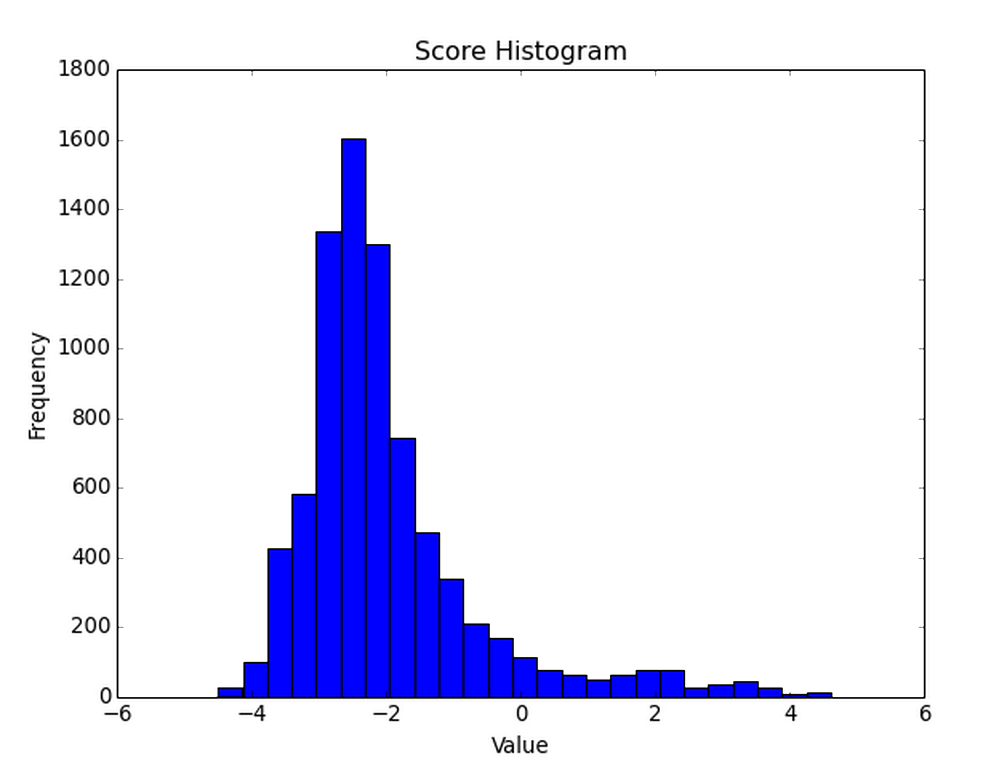
\includegraphics[width=0.6\linewidth]{img/data_hist.png}
  \end{tabular} 
  \caption{Histogram showing the score distribution for the given data} 
  \label{fig:hist_data} 
\end{figure}

% subsection histogram (end)

\subsection{Learning Task} % (fold)
\label{sub:learning_task}
The learning task in this projects is to predict the score for a new tweet. In order to do this we have to ...
% subsection learning_task (end)

\subsection{Pipeline} % (fold)
\label{sub:pipeline}

In order to have a running system where we can use our raw twitter data as an input and get an error value as output, we need to implement a couple of steps. This ends up as a chain of processes, which we defines in a system pipeline model. This model is shown in figure \ref{fig:pipeline}.

\begin{figure}[ht]
\centering 
  \begin{tikzpicture}[node distance=3cm]

  \node (raw) [state] {Raw Data};
  \node (ppc) [process, right of=raw] {Preprocessing};
  \node (ppc_data) [state, right of=ppc] {Processed Data};
  \node (create) [process, right of=ppc_data] {Create Feature Vectors / Representations};
  \node (matrix) [state, below right = 2.5cm and 1.5cm of create] {Feature / Score Matrices};
  \node (fit) [process, below = 6cm of create] {Fit Model To Data};
  \node (sentiment) [state, left of = fit] {Sentiment Predictor};
  \node (acc) [process, left of= sentiment] {Accuracy Assesment};
  \node (error) [state, left of =acc] {Error};

  \node (ppc_desc) [description, below =.5cm of ppc] {Emoticons?\\Spell Check?\\Grammar / Punctuation?\\x\% most common words?\\Verb/Noun/Adjective relations?\\Other considerations ...};

  \node (create_desc) [description, below =.5cm of create] {Emoticons?\\Spell Check?\\Grammar / Punctuation?\\x\% most common words?\\Verb/Noun/Adjective relations?\\Other considerations ...};

  \node (fit_desc) [description, above = .5cm of fit] {SVMs?\\Nalve Bayes?\\Neural Netsn?\\Maximum Entropy?\\Logistic Reg?};

  \node (acc_desc) [description, above = .5cm of acc] {Sum of L1 Error?\\Sum of L2 Error?};



  \draw [arrow] (raw) -- (ppc);
  \draw [arrow] (ppc) -- (ppc_data);
  \draw [arrow] (ppc_data) -- (create);
  \draw [arrow] (create) -- ++ (2,0) -- ++ -| (matrix);
  \draw [arrow] (matrix) -- ++ (0,-2) |- (fit);
  \draw [arrow] (fit) -- (sentiment);
  \draw [arrow] (sentiment) -- (acc);
  \draw [arrow] (acc) -- (error);

  \draw [line] (ppc) -- (ppc_desc);
  \draw [line] (create) --  (create_desc);
  \draw [line] (fit) -- (fit_desc);
  \draw [line] (acc) -- (acc_desc);

  \end{tikzpicture}
  \caption{Pipeline Model} 
  \label{fig:pipeline} 
\end{figure}

% subsection pipeline (end)

\subsection{Evaluation} % (fold)
\label{sub:evaluation}

% subsection evaluation (end)